\section{Background and Problem Setup}\label{background}
This section formalizes the iterative data cleaning and training process and highlights several use-cases and examples.

\subsection{Predictive Modeling}
The user provides a relation $R$ and wishes to train a model using the data in $R$.
This work focuses on a class of well-analyzed predictive analytics problems; ones that can be expressed as the minimization of convex loss functions.
Convex loss minimization problems are amenable to a variety of incremental optimization methodologies with provable guarantees (see Friedman, Hastie, and Tibshirani \cite{friedman2001elements} for an introduction).
Examples include generalized linear models (including linear and logistic regression), support vector machines, and in fact, means and medians are also special cases. 

We assume that the user provides a featurizer $F(\cdot)$ that maps every record $r \in R$ to a feature vector $x$ and label $y$.
For labeled training examples $\{(x_{i},y_{i})\}_{i=1}^{N}$, the problem is to find a vector of \emph{model parameters} $\theta$ by minimizing a loss function $\phi$ over all training examples:
\[
 \theta^{*}=\arg\min_{\theta}\sum_{i=1}^{N}\phi(x_{i},y_{i},\theta)
\]
Where $\phi$ is a convex function in $\theta$.
For example, in a linear regression $\phi$ is:
\[
\phi(x_{i},y_{i},\theta) = \|\theta^Tx_{i} - y_i \|_2^2
\]
Typically, a \emph{regularization} term $r(\theta)$ is added to this problem.
$r(\theta)$ penalizes high or low values of feature weights in $\theta$ to avoid overfitting to noise in the training examples.
\begin{equation}
 \theta^{*}=\arg\min_{\theta}\sum_{i=1}^{N}\phi(x_{i},y_{i},\theta) + r(\theta)
 \label{ideal}
\end{equation}
In this work, without loss of generality, we will include the regularization as part of the loss function i.e., $\phi(x_{i},y_{i},\theta)$ includes $r(\theta)$.

\subsection{Training-Cleaning Iteration}
We consider corruption that affects the attribute values of records and does not cover errors that simultaneously affect multiple records such as record duplication or structure such as schema transformation.
Examples of supported cleaning operations include, batch resolving common inconsistencies (e.g., merging ``U.S.A" and ``United States"), filtering outliers (e.g., removing records with values $>1e6$), and standardizing attribute semantics (e.g., ``1.2 miles" and ``1.93 km").
If there were no data error, $\theta^{*}$ (in Equation \ref{ideal}) would be the optimal model.
The challenge is that if some subset of the rows in $R$ are incorrect or inconsistent, the optimal model will reflect the dirty data (denoted as $\theta^{d}$).
If we were hypothetically able to clean the rows of $R$ before training resulting in $R_{clean}$ and then trained the model, this would result in a model $\theta^{*} \ne \theta^{d}$.

We are particularly interested in those errors that are difficult or time-consuming to clean, and require a human to examine an erroneous record, and determine the appropriate action--possibly leveraging knowledge of the current best model.
We treat the supervisor as an oracle (implemented via human or algorithm) that given a dirty record will return a unique clean record.
We represent this operation as $Clean(\cdot)$ which can be applied to a record $r$ (or a set of records) to recover the clean record $r' = Clean(r)$.
Formally, we treat the $Clean(\cdot)$ as an expensive user-defined function composed of deterministic \textsf{map} and \textsf{filter} operations applied to a subset of rows in the relation.
A relation is defined as \emph{clean} if $R_{clean} = Clean(R_{clean})$.
Therefore, for every $r \in R_{clean}$ there exists a unique $r' \in R$ in the dirty data.
The \textsf{map} and \textsf{filter} cleaning model is not a fundamental restriction of \sys, and Appendix~\ref{set-of-r} discusses a compatible ``set of records" cleaning model.

As an example of how $Clean(\cdot)$ fits into an iterative analysis process, consider an analyst training a regression and identifying outliers. 
When she examines one of the outliers, she realizes that the base data (prior to featurization) has a formatting inconsistency that leads to incorrect parsing of the numerical values.
She applies a batch fix (i.e., $Clean(\cdot)$) to all of the outliers with the same error, and re-trains the model. 
This iterative process can be described as the following pseudocode loop:
\begin{enumerate}[leftmargin=1em]\scriptsize\sloppy
  \item \texttt{Init(iter)}
  \item \texttt{current\_model = Train(R)}
  \item For each t in $\{1,...,iter\}$
  \begin{enumerate}
    \item \texttt{dirty\_sample $=$ Identify(R,current\_model)}
    \item \texttt{clean\_sample $=$ Clean(dirty\_sample)}
    \item \texttt{current\_model $=$ Update(clean\_sample, R)}
  \end{enumerate}
  \item \texttt{Output: current\_model}
  \end{enumerate}

\vspace{0.5em}

Apart from $Train(\cdot)$ and $Clean(\cdot)$, which we have already discussed, the analyst also has to define the primitives $Identify(\cdot)$ and $Update(\cdot)$.
For $Identify(\cdot)$, given a the current best model, the analyst must specify some criteria to select a set of records to examine.
And in $Update(\cdot)$, the analyst must decide how to update the model given newly cleaned data.
It turns out that these primitives are not trivial to implement since the straight-forward solutions can actually lead to divergence of the trained models.

\subsection{Challenges}\label{correctness} 
\vspace{0.5em} 
\textbf{Correctness: } Let us assume that the analyst has implemented an $Identify(\cdot)$ function that returns $k$ candidate dirty records.
The straight-forward application data cleaning is to repair the corruption in place, and re-train the model after each repair.
Suppose $k \ll N$ records are cleaned, but all of the remaining dirty records are retained in the dataset.
Figure \ref{update-arch1} highlights the dangers of this approach on a very simple dirty dataset and a linear regression model i.e., the best fit line for two variables. 
One of the variables is systematically corrupted with a translation in the x-axis (Figure \ref{update-arch1}a).
The dirty data is marked in red and the clean data in blue, and they are shown with their respective best fit lines.
After cleaning only two of the data points (Figure \ref{update-arch1}b), the resulting best fit line is in the opposite direction of the true model.

Aggregates over mixtures of different populations of data can result in spurious relationships due to the well-known phenomenon called Simpson's paradox \cite{simpson1951interpretation}.
Simpson's paradox is by no means a corner case, and it has affected the validity of a number of high-profile studies~\cite{simpsonsparadox}; even in the simple case of taking an average over a dataset.
Predictive models are high-dimensional generalizations of these aggregates without closed form techniques to compensate for these biases.
Thus, training models on a mixture of dirty and clean data can lead to unreliable results, where artificial trends introduced by the mixture can be confused for the effects of data cleaning.

\begin{figure}[ht!]
\centering
 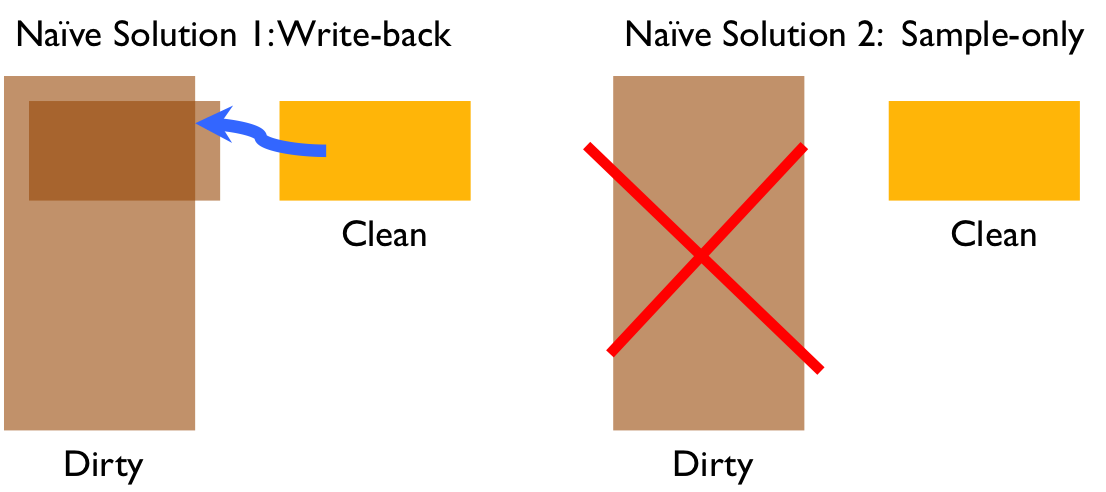
\includegraphics[width=\columnwidth]{figs/update-arch.png}
 \caption{(a) Systematic corruption in one variable can lead to a shifted model. 
 (b) Mixed dirty and clean data results in a less accurate model than no cleaning.
(c) Small samples of only clean data can result in similarly inaccurate models. \label{update-arch1}}
\end{figure}

An alternative is to avoid the dirty data altogether instead of mixing the two populations, and the model re-training is restricted to only data that are known to be clean.
This approach is similar to SampleClean \cite{wang1999sample}, which was proposed to approximate the results of aggregate queries by applying them to a clean sample of data.
However, high-dimensional models are highly sensitive to sample size.
Figure \ref{update-arch1}c illustrates that, even in two dimensions, models trained from small samples can be as incorrect as the mixing solution described before.

\vspace{0.5em} 

\textbf{Efficiency: } Conversely, hypothetically assume that the analyst has implemented a correct $Update(\cdot)$ primitive and implements $Identify(\cdot)$ with a technique such as Active Learning to select records to clean~\cite{yakout2013don,DBLP:journals/pvldb/YakoutENOI11,gokhale2014corleone}.
Active learning is a technique to carefully select the set of examples to learn the most accurate model.
However, these selection criteria are designed for stationary data distributions, an assumption which is not true in this setting.
As more data are cleaned, the data distribution can change leading to evolving criteria of which records are the most valuable to clean.

\subsection{The Need For Automation}\label{alrw}
\sys is a framework that implements the $Identify(\cdot)$ and $Update(\cdot)$ primitives for the analyst. 
By automating the iterative process, \sys ensures reliable semantics on trained models.
The analyst initializes \sys with a dirty model.
\sys carefuly selects small batches of data to clean based on data that are likely to be dirty and likely to affect the model.
The analyst applies data cleaning to these batches, and \sys updates the model with an incremental optimization technique.

Machine learning has been applied in prior work to improve the efficiency of data cleaning~\cite{yakout2013don,DBLP:journals/pvldb/YakoutENOI11,gokhale2014corleone}.
Human input, either for cleaning or validation of automated cleaning, is often expensive and impractical for large datasets.
A model can learn rules from a small set of examples cleaned (or validated) by a human, and active learning is a technique to carefully select the set of examples to learn the most accurate model.
This model can be used to extrapolate repairs to not-yet-cleaned data, and the goal of these approaches is to provide the cleanest possible dataset--independent of the subsequent analytics or query processing.
These approaches, while very effective, suffer from composibility problems when placed inside cleaning and training loops.
To summarize, \sys considers data cleaning \emph{during} model training, while these techniques consider model training \emph{for} data cleaning.
One of the primary contributions of this work is an incremental model update algorithm with correctness guarantees for mixtures of data.

\subsection{Use Case: Dollars for Docs \cite{dollarsfordocs}}\label{s:usecase}
ProPublica collected a dataset of corporate donations to doctors to analyze conflicts of interest. 
They reported that some doctors received over \$500,000 in travel, meals, and consultation expenses \cite{dollarsfordocsa}.
ProPublica laboriously curated and cleaned a dataset from the Centers for Medicare and Medicaid Services that listed nearly 250,000 research donations, and aggregated these donations by physician, drug, and pharmaceutical company.
We collected the raw unaggregated data and explored whether suspect donations could be predicted with a model.
This problem is typical of analysis scenarios based on observational data seen in finance, insurance, medicine, and investigative journalism.
The dataset has the following schema:
\begin{lstlisting}[mathescape,basicstyle={\scriptsize}]
Contribution(pi_specialty$\textrm{,}$ drug_name$\textrm{,}$ device_name$\textrm{,}$
corporation$\textrm{,}$ amount$\textrm{,}$ dispute$\textrm{,}$ status)
\end{lstlisting}

\noindent\texttt{pi\_specialty} is a textual attribute describing the specialty of the doctor receiving the donation.

\noindent\texttt{drug\_name} is the branded name of the drug in the research study (null if not a drug).

\noindent\texttt{device\_name} is the branded name of the device in the study (null if not a device).

\noindent\texttt{corporation} is the name of the pharmaceutical providing the donation.

\noindent\texttt{amount} is a numerical attribute representing the donation amount.

\noindent\texttt{dispute} is a Boolean attribute describing whether the research was disputed.

\noindent\texttt{status} is a string label describing whether the  donation was allowed under the declared research protocol. The goal is to predict disallowed  donation. 

\vspace{0.5em}

However, this dataset is very dirty, and the systematic nature of the data corruption can result in an inaccurate model.
On the ProPublica website \cite{dollarsfordocs}, they list numerous types of data problems that had to be cleaned before publishing the data (see Appendix \ref{dfd-errors}).
For example, the most significant donations were made by large companies whose names were also more often inconsistently represented in the data, e.g., ``Pfizer Inc.", ``Pfizer Incorporated", ``Pfizer".
In such scenarios, the effect of systematic error can be serious.
Duplicate representations could artificially reduce the correlation between these entities and suspected contributions.
There were nearly 40,000 of the 250,000 records that had either naming inconsistencies or other inconsistencies in labeling the allowed or disallowed \texttt{status}.
Without data cleaning, the detection rate using a Support Vector Machine was 66\%.
Applying the data cleaning to the entire dataset improved this rate to 97\% in the clean data (Section \ref{dfd-exp}), and the experiments describe how \sys can achieve an 80\% detection rate for less than 1.6\% of the records cleaned.


%\sys avoids both pitfalls, Simpson's paradox and sample size dependence.

\iffalse
\sys avoids both pitfalls, Simpson's paradox and sample size dependence.
In Section \ref{model-update}, we show how we do this with iterative gradient steps (i.e., incrementally moving the line based on the clean data).
This takes advantage of the dirty data as well as the clean data, but still have provable properties about the intermediate results.
The intuition is that it smoothly and iteratively transitions the model from one population (the dirty data) to another (the clean data).
In Figure \ref{sys-arch2}, we illustrate our ideal tradeoff space of sampling and data cleaning.
At two extremes we have no cleaning (just using the dirty data) and full cleaning.
%\sys is optimized for convergence for smaller sample sizes than a uniform sampling approach.

\begin{figure}[t]
\centering
 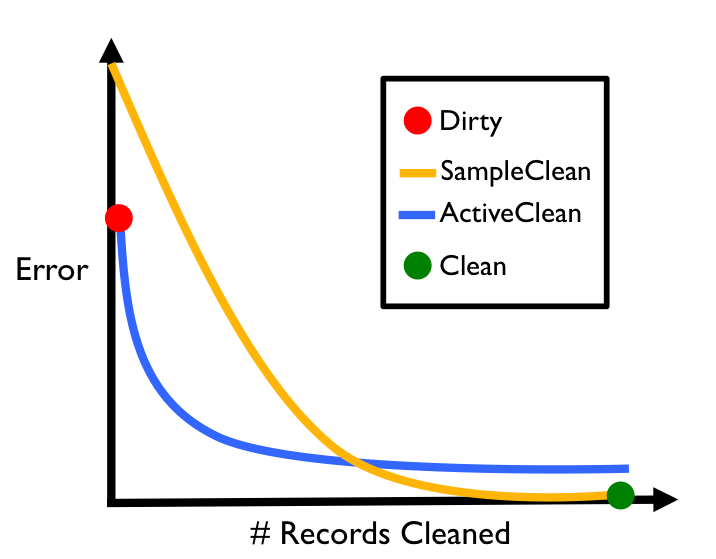
\includegraphics[width=0.5\columnwidth]{figs/arch2.png}
 \caption{\sys is designed to converge to an accurate model with fewer cleaned records than a uniform sampling approach (SampleClean). \label{sys-arch2}}\vspace{-1em}
\end{figure}


We design \sys to make greater progress at these small sample sizes using the dirty model as an initialization.
Doing so is not trivial since it requires analysis of both the Machine Learning model and the data cleaning operations.
Data may look unimportant to a dirty model but when cleaned are very important.
Also, data cleaning and model training can happen at very different time scales, we have to carefully budget our effort to ensure that any optimizations actually address rate-determining steps in the workflow.
Finally, in this line of work, the tradeoff space is enormous, and we have to carefully pick a design point and tailor our optimizations to this preferred regime.
\fi

%Consider the data corruption in our motivating example where company names were inconsistently entered: ``Pfizer Inc.", ``Pfizer Incorporated", ``Pfizer".
%Fixing this error can be represented as a record-by-record mapping.
%The data cleaning function would pick one canonical representation for the company (e.g. ``Pfizer Inc.") and map all records with other values that refer to the same real-world entity to the canonical representation.
%However, there are types of data cleaning that do not satisfy this model such as schema mapping, record deduplication, and data extractions that create additional columns. 


